\section{Arbres de calcul (6 points)}

\begin{questions}
	\question[3] Décrire par une phrase les arbres de calcul suivant et écrire l'expression correspondante (le résultat n'est pas demandé).
	
	
	\begin{center}
		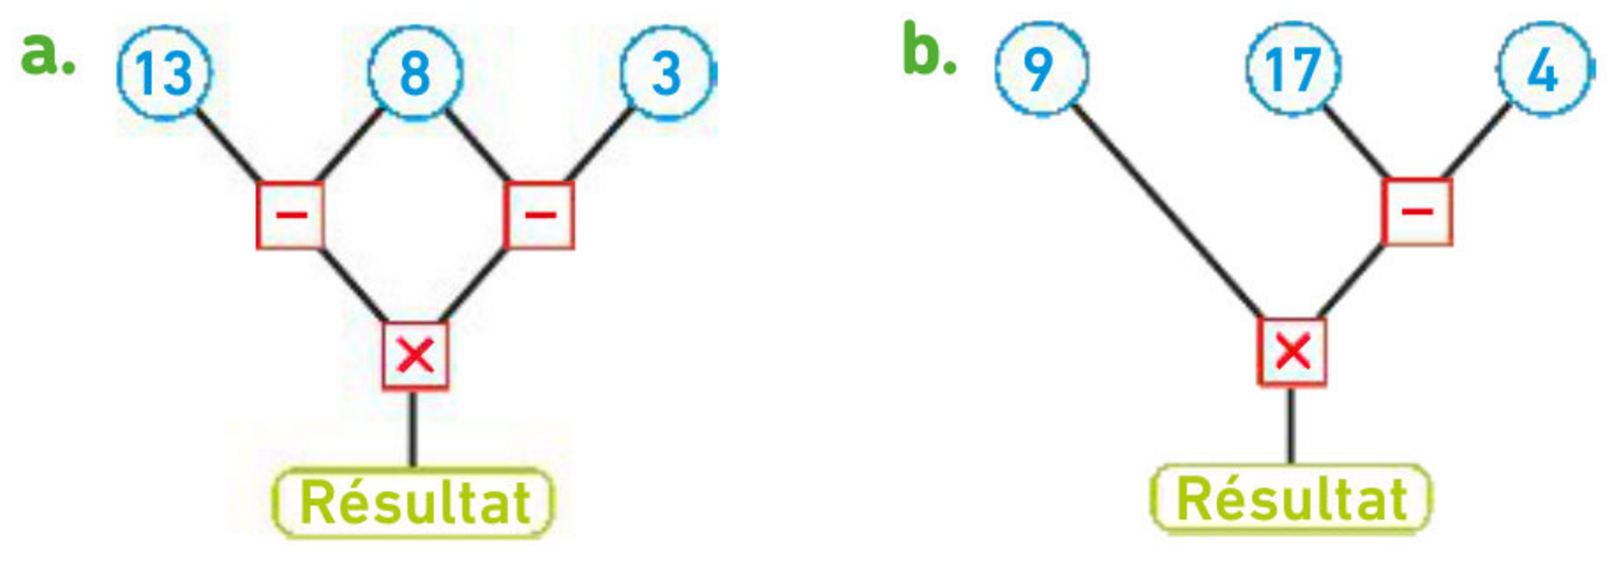
\includegraphics[scale=0.3]{img/arbres}
	\end{center}
	
	\begin{solution}
		\begin{enumerate}
			\item Cet arbre correspond au produit de la différence de 13 et 8 et de celle de 8 et 3. ($(13 - 8) \times (8 - 3)$).
			
			\item Cet arbre correspond au produit de 9 par la différence de 17 et 4. ($9 \times (17 - 4)$).
		\end{enumerate}
	\end{solution}
	\question[3] Décrire par une phrase les expressions suivantes et dessiner l'arbre de calcul correspondant.
	
	\begin{multicols}{2}
		\begin{enumerate}
			\item $30 \times 4 + 20 \div 2$
			\item $30 \times (20 - 4)$
			%\item $10 + 4 \times 10$
		\end{enumerate}
	\end{multicols}	

	
	\begin{solution}
		\begin{multicols}{2}
			\begin{enumerate}
				\item Cette expression correspond à la somme du produit de 30 et 4 et du quotient de 20 par 2.
					
				\item Cette expression correspond au produit de 30 par la différence de 20 et 4.
			\end{enumerate}
		
		\end{multicols}
	\end{solution}
	
\end{questions}
